\documentclass[french]{article}
\usepackage[T1]{fontenc}
\usepackage[utf8]{inputenc}
\usepackage{lmodern}
\usepackage[a4paper]{geometry}
\usepackage{babel}
\usepackage{amsmath}
\usepackage{amsfonts}
\usepackage{tcolorbox}
\usepackage{color}
\usepackage{breqn}

\usepackage{tikz}
\usetikzlibrary{angles,quotes}

\begin{document}
	\title{DM4: Oscillateur harmonique}
	\author{Gabriel PEREIRA DE CARVALHO}
	\date{Dernière modification \today}
	
	\maketitle
	
	\subsection*{Exercice 1}
	
	D'abord, faisons un diagramme du problème.
	
	\begin{center}
		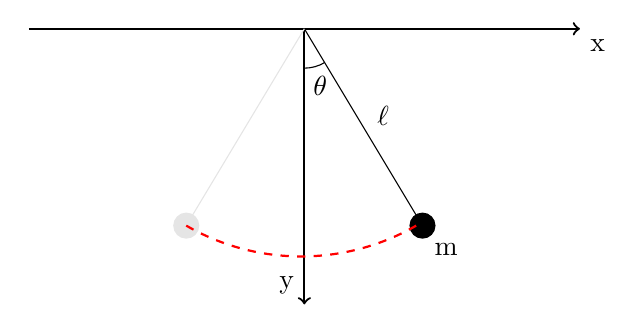
\begin{tikzpicture}
			\coordinate (centro) at (0,0);
			\coordinate (particle) at (1.5, -2.5);
			\coordinate (particlelabel) at (1.8, -2.8);
			\coordinate (linelabel) at (1, -1.1);
			\coordinate (symparticle) at (-1.5, -2.5);
			\coordinate (ylim) at (0, -3.5);
			
			\draw[thick,->] (-3.5,0) -- (3.5,0) node[anchor=north west] {x};
			\draw[thick,->] (0,0) -- (0, -3.5) node[anchor=south east] {y};
			
			\draw (centro) -- (particle) node[fill,circle](m){};
			\draw[black!10] (centro) -- (symparticle) node[fill, circle](m){};
			\node at (particlelabel) {m};
			\node at (linelabel) {$\ell$};
			
			\pic[draw,angle radius=.5cm,angle eccentricity=1.5,"$\theta$"] {angle=ylim--centro--particle};
			\draw[red,thick,dashed] (symparticle) arc (240:300:2.92cm);
		\end{tikzpicture}
	\end{center}

	Alors, calculons l'énergie cinétique et l'énergie potentielle de la masse
	\begin{align}
		\begin{cases}
			T &= \frac{m \ell^2 \dot{\theta}^2}{2}\\
			V &= -mg \ell \cos\theta
		\end{cases}
	\end{align}
	
	\subsection*{Exercice 2}
	
	On a le Lagrangien
	
	\begin{equation}
		\mathcal{L} = T - V = \frac{m \ell^2 \dot{\theta}^2}{2} + mg \ell \cos\theta
	\end{equation}
	
	\subsection*{Exercice 3}
	
	Par l'équation d'Euler-Lagrange, on a
	
	\begin{equation}
		\frac{d}{dt} \left(\frac{\partial}{\partial \dot{\theta}} \mathcal{L}\right) = \frac{\partial}{\partial \theta} \mathcal{L} \iff m \ell^2 \ddot{\theta} = -mg\ell \sin\theta \iff \ddot{\theta} = -\frac{g}{\ell} \theta
	\end{equation}
	
	Alors utilisons l'approximation pour des petits angles $\sin \theta \approx \theta$ et posons $\omega^2 = \frac{g}{\ell}$, on a
	
	\begin{equation}
		\ddot{\theta} = -\omega^2 \theta
	\end{equation}
	
	l'équation pour un oscillateur harmonique classique.
	
\end{document}